\section{Synthesis of the equivalent transmi,ssion for full pupil illumination}
\label{sec:discussion}

Both the telescope reflectivity and filter transmission display a very
clear radial dependency. While the latter is expected due the
interferometric nature of the filters, the origin of the former is not
yet understood. We can nevertheless build an empirical model assuming
smooth transitions between the measurements, and compute from there a
theoretical "full pupill" transmission by averaging the model over the
illuminated portion of the primary mirror. As is demonstrated in Table
TX, these two steps are necessary to reach sub-percent accuracy in
colors and sub-nm accuracy in central wavelengthes. Last we proceed
with propagating the statistical and systematic errors on the final
transmission curves. The impact of these errors in the interpretation
of broadband photometry is better understood when integrated as errors
on the filter normalisation and central wavelength, which can readily
be translated in errors in colors and color-terms.


\subsection{Radial model of the instrument transmission}
\label{sec:model}

The open transmission of the telescope is modeled as a smooth fonction
of wavelength and incidence angle. The function is developped on a 2D
cubic B-spline basis, with \num{35} wavelength nodes regularly spaced
between \SIrange{350}{1100}{nm}, and 2 nodes in angles between
\SI{1.97}{\degree} and \SI{7.24}{\degree}. The two angles corresponds
to the inner and outer edge of the occultation free primary mirror,
set at \SIrange{55}{203}{mm} in radius assuming a \SI{1600}{mm} focal
length.

For data acquired with a filter in the path, the open transmission
model is multiplied by a model of the interference filter transmission
build as follows:
\begin{equation}
  \label{eq:filtertransmission}
T(\lambda, \theta) = \mathcal T\left(\frac{\lambda}{\sqrt{1 -
    (\sin(\theta) / n_\text{eff})^2}}\right)
\end{equation}
where $n_\text{eff}$ is an effective index for the inserted filter,
and $\mathcal T$ is a piece-wise linear function of wavelength. The
piece-wise linear function is first developped on a regular grid with
\num{150} nodes between \SIrange{350}{1100}{nm}, giving a general
resolution of \SI{5}{nm} and is then further refined where needed by
equally splitting in two intervall where the local mean chi-square
exceeds the global mean chi-square by more than $3$ standard
deviations. This refinement process is repeated \num{4} times so that
filter fronts typically end-up being modeled with up to \SI{\sim
  0.3}{nm} resolution.

Last, photometry of the grating zeroth and first orders are adjusted
with the open transmission multiplied by a cubic B-spline decomposed
on 105 nodes in wavelength.

The composite model is fit to dataset number 2, encompassing data at 4
different radii and successive observations without filters and with
all 7 filters and grating. The baseline model has \num{1979} free
parameters, \num{148} to describe the open transmission, \num{420} to
describe each of the grating order, and about $6\times165$ to describe
each of the $ugrizy$ filters. The $u$ band filters blue edge cannot be
reliably determined by the data. Fit results are shown in
Fig.~\ref{fig:lambdathetafitresults}.

\begin{figure*}
  \centering
  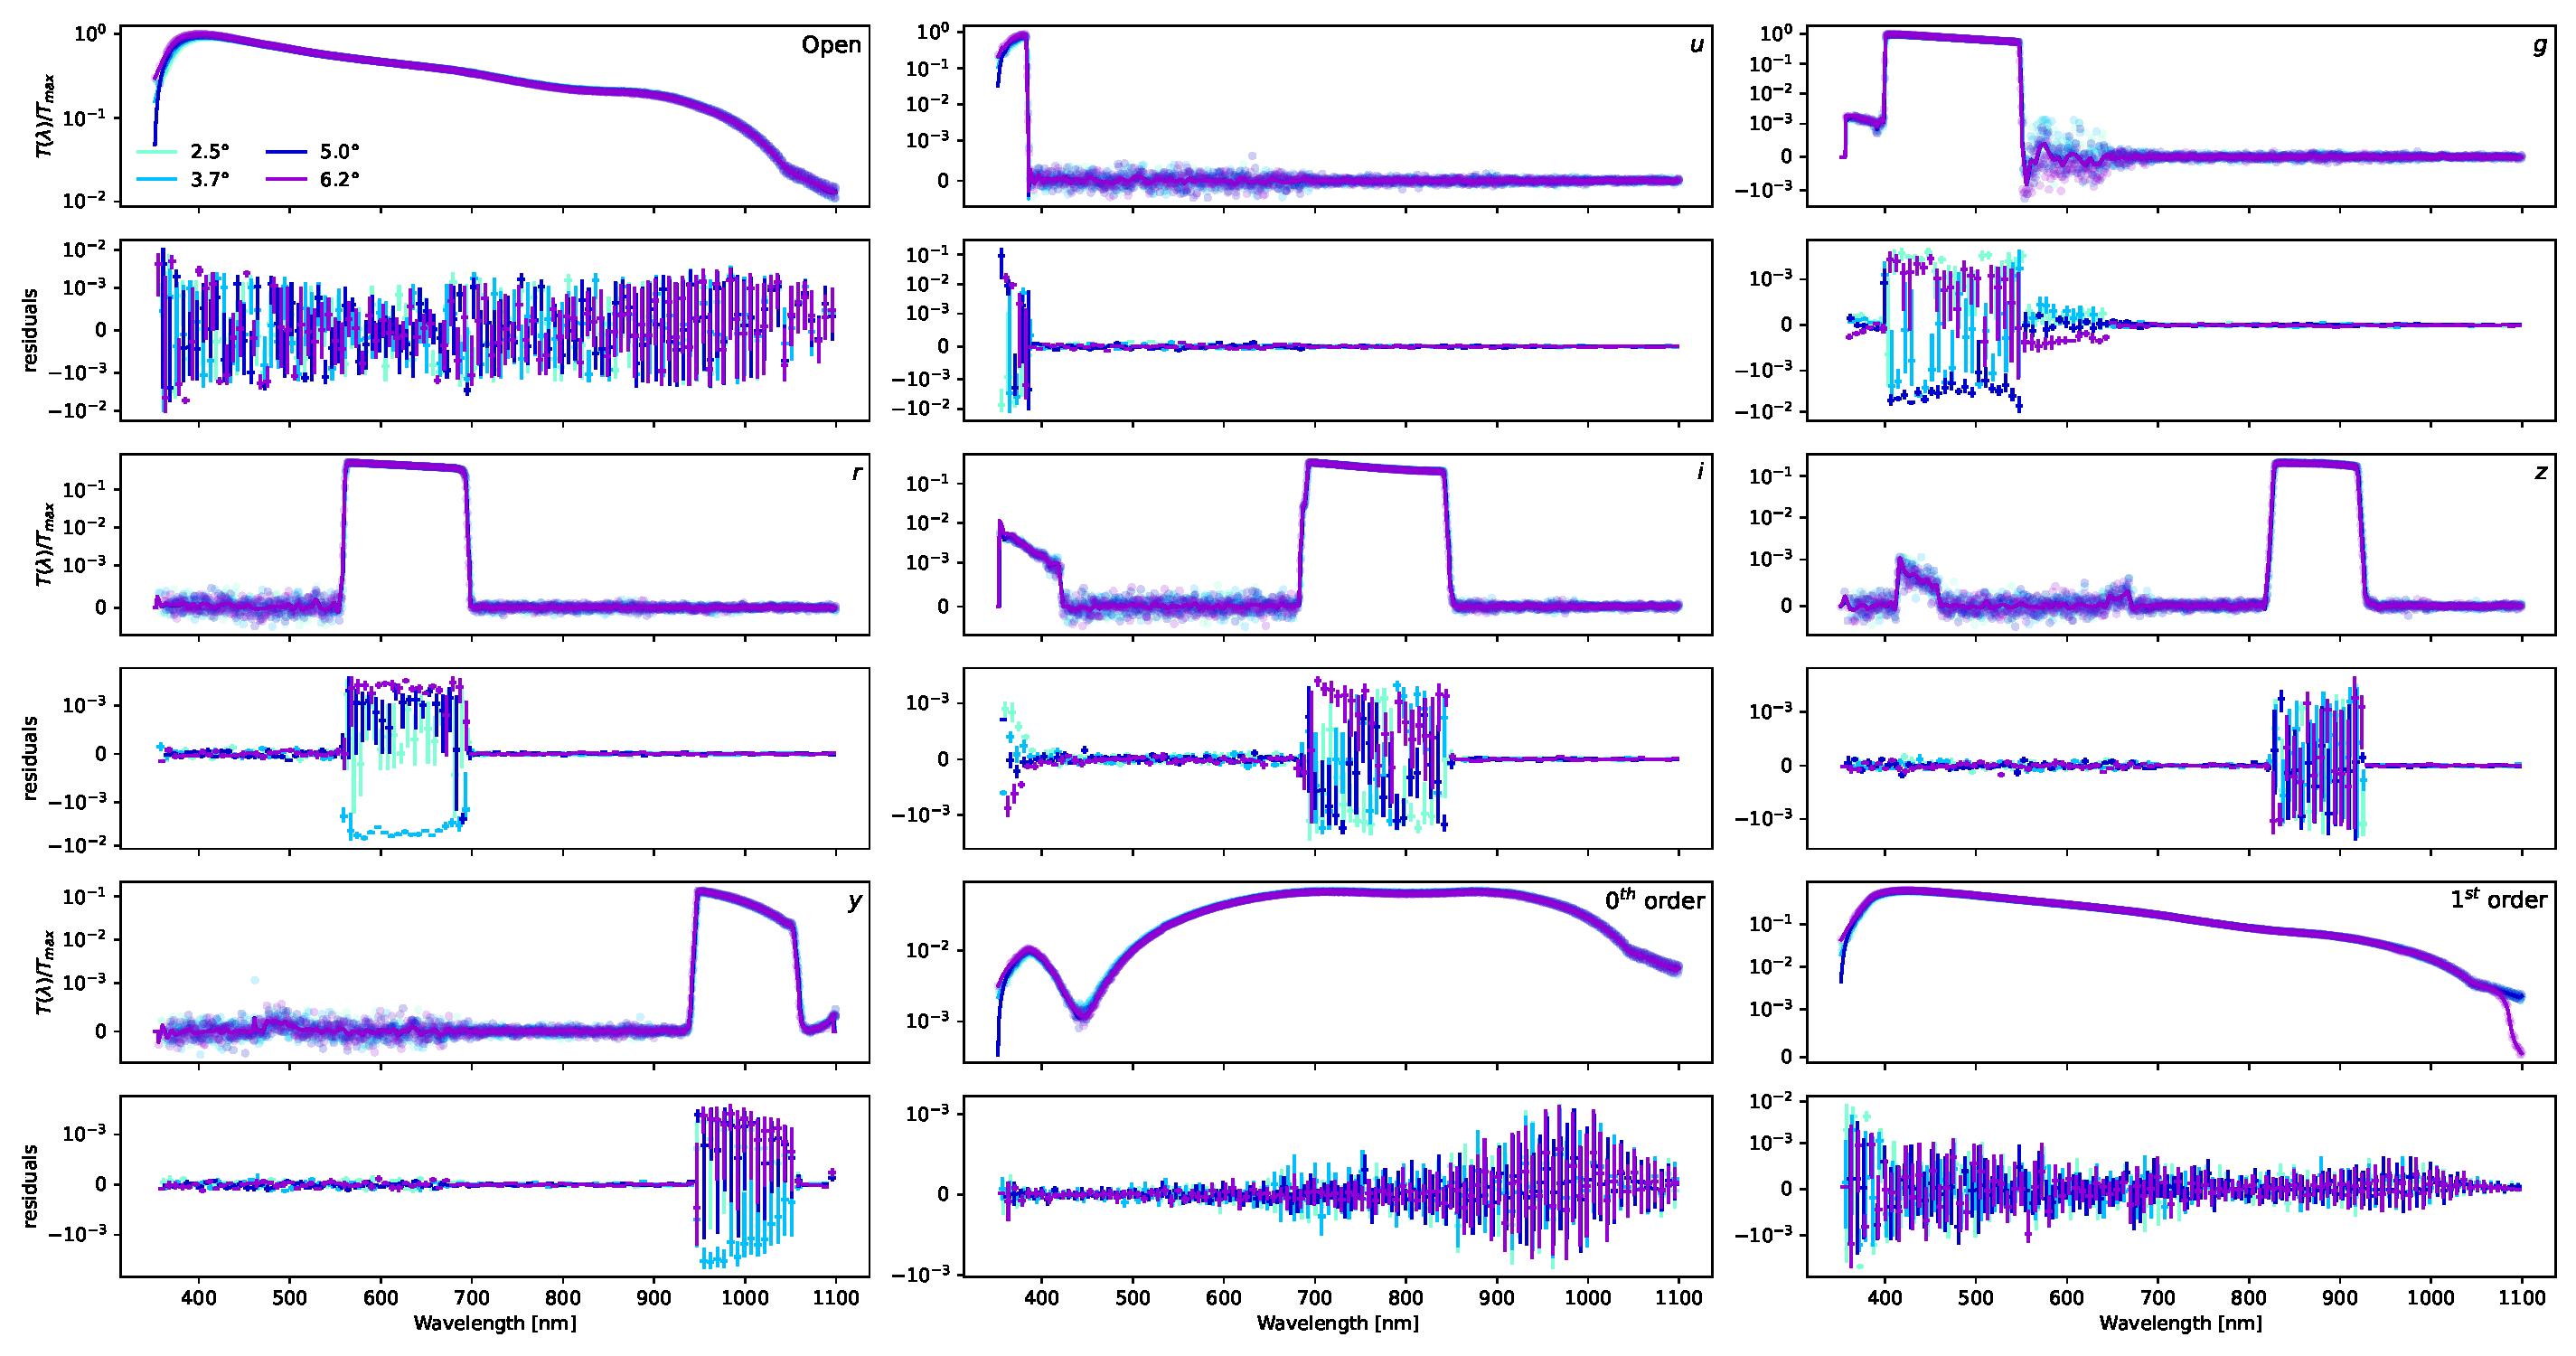
\includegraphics[width=1\linewidth]{./fig/lambdathetafitresults.pdf}
  \caption{Model of the wavelength and radial dependency of the
    StarDICE response to CBP illumination $R(\lambda)$ (see
    Eq.~\ref{eq:rtot}). Each pannel display the raw measurements at
    the 4 sampled position for each of the filter configurations: no
    filters (Open), with one of the 6 photometric filters ($ugrizy$)
    or with the grating looking either at the zeroth order or the
    first order spots. The pannel immediately below each pannel
    display the residuals to the model. All pannels are normalized to
    the peak of the response, reached in the open configuration at
    \SI{398}{nm} and \SI{6.2}{\degree}.  }
  \label{fig:lambdathetafitresults}
\end{figure*}

The model satisfactorilly describes the dataset. The most significant
discrepancy is a noticeable gray decrease of the transmission of the
$r$ filters for the sample measurement at \SI{3.7}{\degree} with
respect to the average of the other three. Investigating this issue,
we found that the PSF tails in the corresponding images display a
diffraction figure consistent with the beam being intercepted by a
dust particle on the filter surface with a diameter in the range
\SIrange{200}{300}{\micro\meter}. The approximate area of the beam
spot being \SI{12}{mm\squared}, the estimated particule sizes predicts
a decrease in transmission of up to \SI{0.6}{\percent}, very
consistent with the observed decrease. Very similar decrease are
observed for some observations in $u,g$ and $y$. Although in these
cases it was not possible to estimate the particule size from
diffraction features in the images, we think that similar dust
contamination is at play. The size of the ``gray'' discrepancies are
easier to read on the top pannel of Fig.~\ref{fig:metrics}, which
displays the difference in the transmission integral between the
measurement and the model at each position. The standard deviation of
the model/measurement discrepancies is \SI{10.2}{mmag}. Taking this
number as an estimate of dust-induced dispersion, we can deduce that
the corresponding uncertainty on the per-filter normalisation of the
model, which average 4 independant samples, is of the order of
\SI{5}{mmag}.

The bottom panel in Fig.~\ref{fig:metrics} displays the difference in
central wavelength between the model and the measurement for all 4
radius in the central panel of Fig.~\ref{fig:metrics}. The model
successfully reproduces the central wavelength of all filters with a
standard deviation of \SI{0.13}{nm} which delivers an improvement by
an order of magnitude with respect to a model neglecting the
wavelength shift. 

\begin{figure}
  \centering
  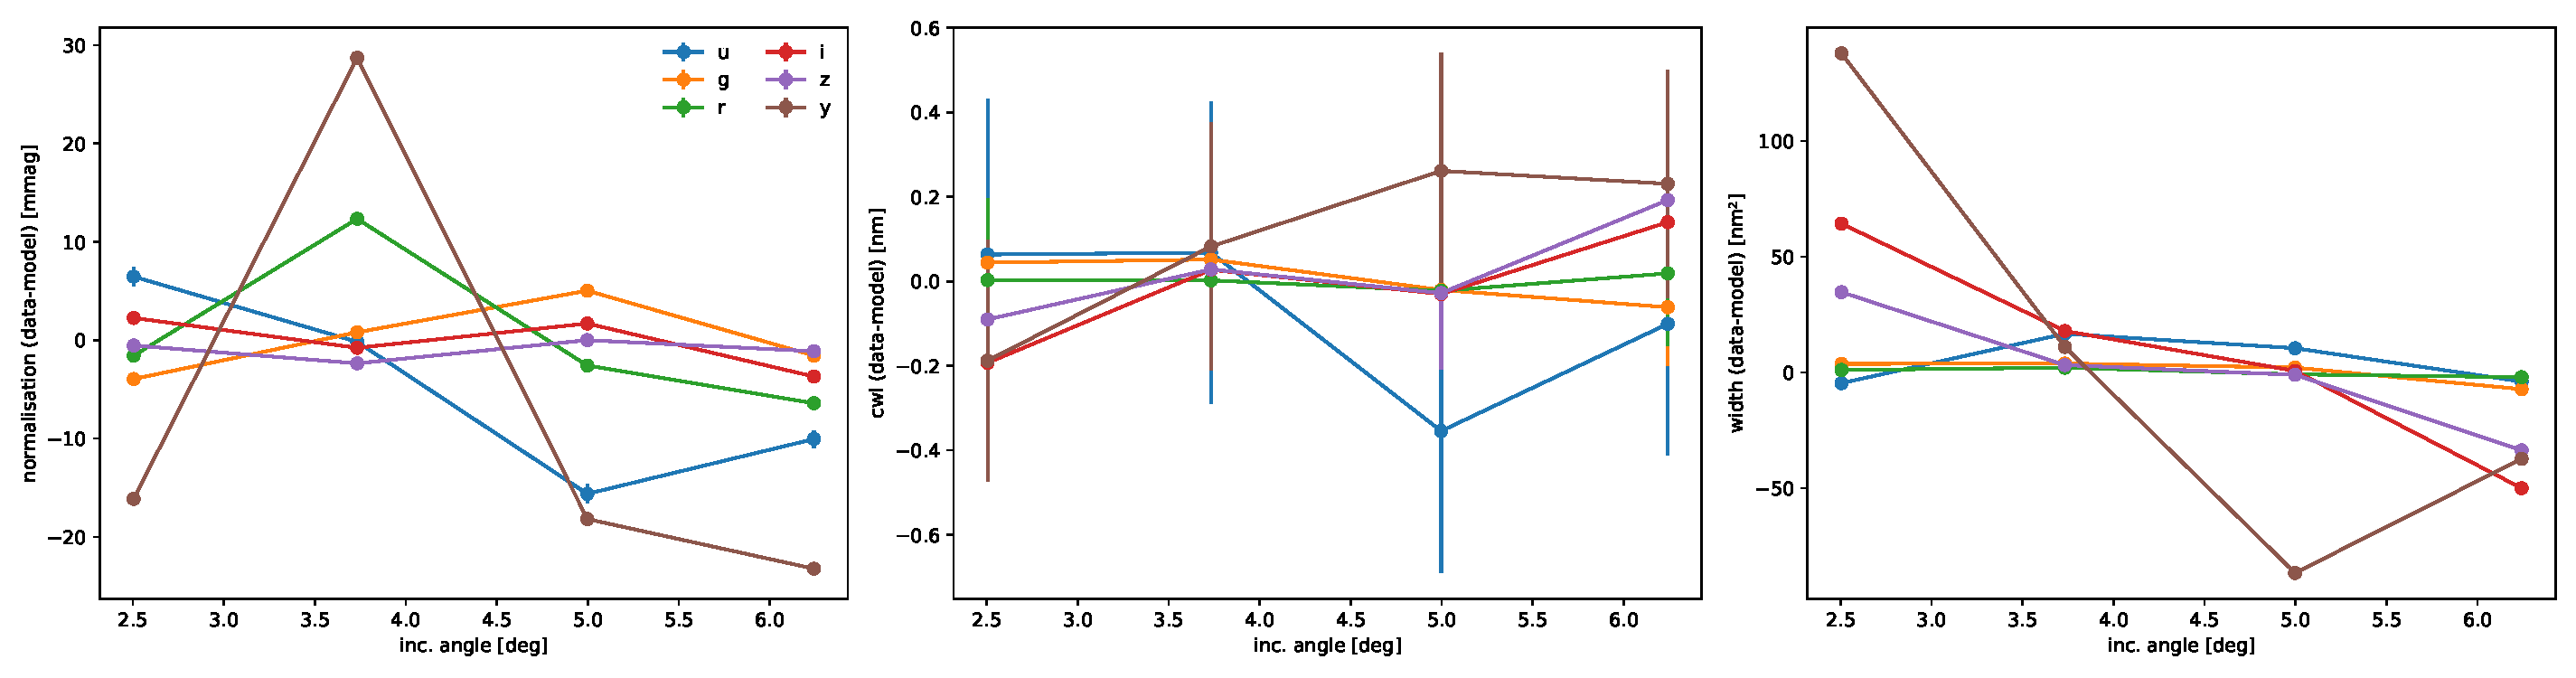
\includegraphics[width=1\linewidth]{fig/metrics.pdf}
  \caption{Discrepancies between model and raw measurements at different mirror locations summarized according to 3 metrics: summarize}
  \label{fig:metrics}
\end{figure}

\subsection{Full pupil synthetic transmission curves}

The full pupil transmission is synthesized by numerically averaging
the above model assuming that the pupil is a perfect annulus with an
inner radius of \SI{55}{mm} and an outer radius of \SI{203}{mm}. A
rectangular quadrature with 100 evenly sampled points in radius has
been used for the averaging. The curves have been normalized using the
CBP response from Sect. (corrected for the \SI{5}{mm} to
\SI{75}{\micro\meter} pinhole response change determined in Sect. TX.,
and the aperture fraction estimated in Sect.Tx).  An estimate of the
absolute transmission curve is then computed assuming an effective
mirror area of TX. The resulting transmission curves are shown in
Fig.~\ref{fig:fullpupiltrans}.
\begin{figure}
  \centering
  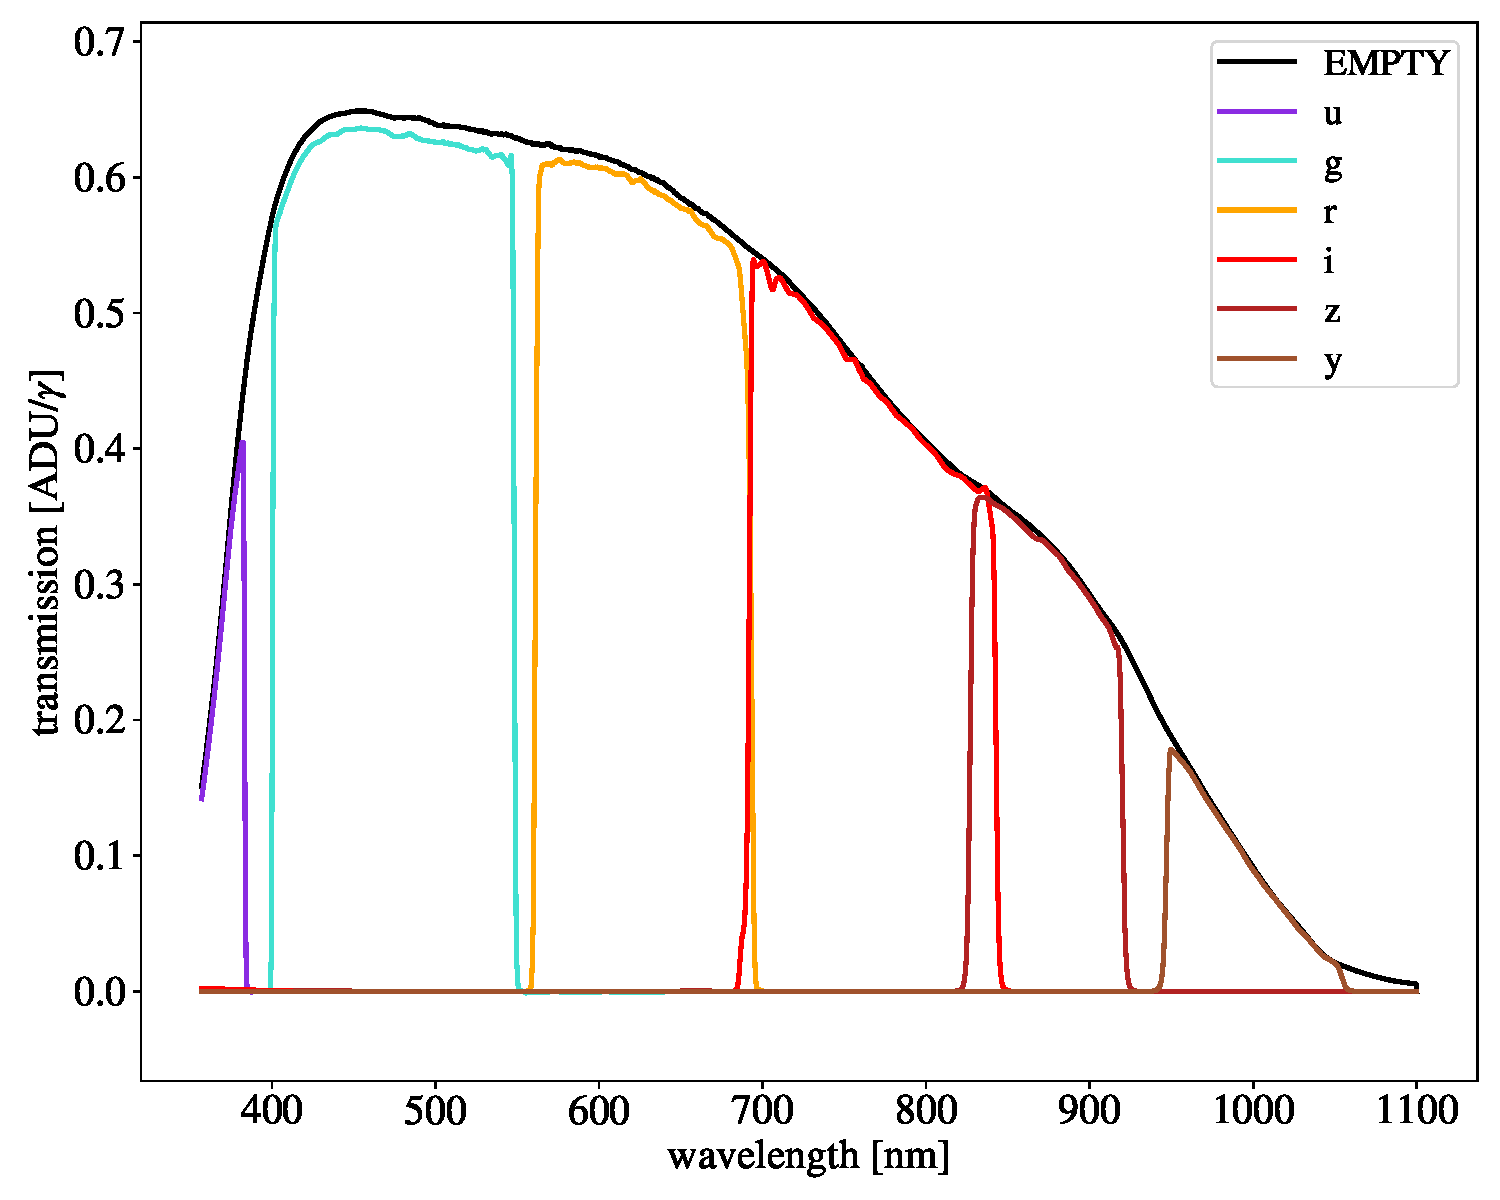
\includegraphics[width=1\linewidth]{fig/fullpupill.pdf}
  \caption{Full-pupill transmission curves for the StarDICE instruments.}
  \label{fig:fullpupiltrans}
\end{figure}

\todo{
We also tested the model against the 4 remaining mirror samples that
are not part of the training dataset. The result of the test is
summarized in Fig.\ref{fig:metrics}.}


\subsection{Final error budget}
